
\chapter{Общая характеристика научного доклада}

\section{Актуальность темы исследования}

Беспилотные летательные аппараты (БЛА) мультироторного типа находят всё более широкое применение в различных областях человеческой деятельности, а миниатюризация и доступность электронных компонентов их бортового оборудования приводит к расширению спектра задач, в решении которых используются такие аппараты.
Интерес исследователей к БЛА обусловлен также и тем, что они являются доступным средством для отработки новых технологий в аэрокосмической отрасли \cite{Otero01}.
С момента создания первых квадрокоптеров интенсивно ведутся исследования в области их динамики и управления, причём количество работ растет с каждым годом, что можно наблюдать по динамике количества публикаций (рис. \ref{pic:res_amount}), посвященных квадрокоптерам, доступных на крупнейшей онлайн платформе научных публикаций «Google Академия».
Однако, несмотря на обилие публикаций, в области управляемой динамики квадрокоптеров остаются перспективные направления, среди которых усовершенствование конструкции БЛА, связанное с увеличением размерности вектора управляющих воздействий.
Конструктивно это достигается, например, с помощью сервоприводов, способных поворачивать роторы с пропеллерами относительно корпуса.
\begin{figure}[h!]
	\centering
	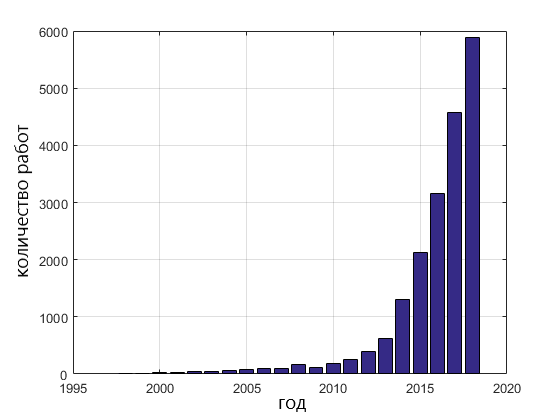
\includegraphics[width=0.95\columnwidth]{res_amount}
	\caption{ -- Динамика количества публикаций, посвященных квадрокоптерам}
	\label{pic:res_amount}
\end{figure}

Стандартный квадрокоптер с четырёхмерным вектором управляющих воздействий и шестью степенями свободы корпуса аппарата не способен, например, независимо управлять положением и ориентацией.
Это приводит к необходимости дополнительных устройств для наведения камер или лазерных дальномеров, используемых при выполнении ряда стандартных для БЛА задач.
Возможность независимо управлять положением и ориентацией, приобретаемая за счёт использования поворотных роторов, влияет не только на работу полезной нагрузки и датчиков, но и на функциональные возможности всей системы в целом.
Согласно работе \cite{Stolc01} усовершенствованные таким образом квадрокоптеры более устойчивы к возмущениям внешней среды, а также лучше стандартных квадрокоптеров пригодны для вертикального взлёта и посадки на неровные поверхности.
Достоинства БЛА с поворотными роторами отмечают и исследователи, работающие над управлением БЛА в экстренных ситуациях (при отказе части двигателей) \cite{Morozov01, Shidar00}.
В работе \cite{Shidar00} обосновывается достижение более высокой скорости за счёт выбора оптимальной по отношению к набегающему потоку ориентации, а также более рациональное по сравнению со стандартными аппаратами энергопотребление.
В работе \cite{Morozov01} отмечена перспективность конструкции с поворотными роторами, однако её применение не рассматривается из-за сложности реализации.
Использование поворотных роторов действительно усложняет реализацию контура управления \cite{Ryll01, Falconi01, Segui01, Oosedo01} и не позволяет применять ставшую классической изящную схему управления \cite{Mellinger01}, однако, есть основания полагать, что предлагаемое в данной работе аналитическое обращение динамики системы позволит преодолеть некоторую часть возникающих трудностей.

\section{Цели и задачи исследования}

Объектом исследования является система управления движением квадрокоптера с поворотными роторами, предметом исследования -- динамика и методы управления движением квадрокоптера с поворотными роторами.

Цель работы -- выполнить анализ динамики квадрокоптера с поворотными роторами;
разработать алгоритмы управления движением квадрокоптера с поворотными роторами для выполнения различных манёвров; разработать алгоритмы управления движением квадрокоптера с поворотными роторами для экстренного сценария -- потере двух смежных двигателей. Для достижения цели работы необходимо решить следующие задачи:
\begin{enumerate}
	\item Разработать математическую модель движения квадрокоптера с поворотными роторами с учётом сил и моментов, действующих на все составные части системы.
	\item Решить задачу обратной динамики и синтезировать контур управления квадрокоптером с поворотными роторами для независимого управления положением и ориентацией аппарата с учётом физических ограничений, накладываемых на исполнительные органы системы управления.
	\item Обеспечить обратную связь в контуре управления, реализовать алгоритмы оценки состояния на основе фильтра Калмана.
	\item Реализовать в синтезированном контуре алгоритм управления положением и ориентацией аппарата, позволяющий совершать сложные манёвры, как, например, отслеживание подвижного объекта с помощью жестко закрепленной бортовой камеры.
	\item Реализовать алгоритмы управления квадрокоптером с поворотными роторами в случае отказа двух смежных двигателей, позволяющие аппарату выполнение номинальных задач.
\end{enumerate}
Для решения сформулированных задач используются классические методы механики, управления, вычислительной и высшей математики.

Область данного исследования соответствует пунктам «Баллистическое проектирование летательных аппаратов различного назначения» и «Динамическое проектирование управляемых летательных аппаратов и исследование динамики их движения» паспорта специальности «05.07.09 – Динамика, баллистика, управление движением летательных аппаратов».

\section{Положения, выносимые на публичное представление}
Положения, выносимые на публичное представление:
\begin{enumerate}
\item Математическая модель управляемой динамики квадрокоптера с поворотными роторами с учётом сил и моментов, действующих на все составные части системы;
\item Синтез контура управления квадрокоптером с поворотными роторами для независимого управления положением и ориентацией; 
\item Алгоритм для учёта физических ограничений, накладываемых на исполнительные органы системы управления;
\item Алгоритм идентификации аэродинамических параметров пропеллеров;
\item Алгоритмы экстренного управления квадрокоптером с поворотными роторами в случае отказа двух смежных двигателей.
\item Выводы и рекомендации, сформулированные в работе.
\end{enumerate}

\section{Степень достоверности и апробация результатов}
Достоверность полученных научных положений, результатов и выводов обеспечивается
соответствием выбранных моделей движения общепринятым стандартам,
адекватностью выбранных методов исследования движения,
проведением численного моделирования полученных аналитических результатов,
а также сопоставлением с результатами,
полученными другими авторами для частных случаев рассматриваемых задач.

Основные научные положения и результаты работы докладывались и обсуждались на 
\begin{itemize}
\item Всероссийской конференции молодых ученых-механиков, 5 - 15 сентября 2017 г., г. Сочи, «Буревестник» МГУ;
\item Международной научной конференции «Фундаментальные и прикладные задачи механики», 24 - 27 октября 2017 г., г. Москва;
\item 60-й Всероссийской научной конференции МФТИ, секция теоретической механики, 20–26 ноября 2017 г., г. Долгопрудный;
\item 60-й Всероссийской научной конференции МФТИ, секция управления динамическими системами, 20–26 ноября 2017 г., г. Москва;
\item седьмой международной конференции «Geometry, Dynamics, Integrable Systems», 5-9 июня 2018 г., г. Москва;
\item XIV Международной конференции «Устойчивость и колебания нелинейных систем управления» (конференция Пятницкого) Россия, Москва, ИПУ РАН, 30 мая -- 1 июня 2018 г.
\item 14-ой международной конференции «Vibration engineering and technology of machinery», 10-13 сентября 2018 г., г. Лиссабон, Португалия;
\item Международной конференции «Проблемы механики и управления», 16-22 сентября 2018 г., г. Махачкала;
\item XXI конференции молодых ученых «Навигация и управление движением», 19–22 марта 2019 г., г. Санкт-Петербург.
\end{itemize}
По теме исследования были опубликованы 10 работ, список можно найти на странице \pageref{list_chapter}.

\section{Научная новизна и практическая значимость работы}
Научная новизна представленных в диссертации результатов заключается в следующем:
\begin{enumerate}
	\item  Получено аналитическое решение задачи обратной динамики БЛА с поворотными роторами;
	\item  Проведен анализ аналитического решения задачи обратной динамики  БЛА с поворотными роторами, разработан алгоритм реализации ограничений на компоненты вектора управляющих воздействий;
	\item  Разработаны алгоритмы экстренного управления квадрокоптером с поворотными роторами в случае отказа двух смежных двигателей.
\end{enumerate}

Практическая значимость работы состоит в том, что
реализация разработанной в исследовании системы управления позволяет проектировать БЛА с улучшенными относительно стандартных квадрокоптеров лётными характеристиками, в том числе обладающих способностью 
выполнять сложные манёвры, недоступные стандартным квадрокоптерам, такие, как манёвры с требованием независимого управления положением и ориентацией.
Таким образом, расширяются возможности беспилотных летательных аппаратов.
Кроме этого, реализованная в программных алгоритмах динамическая модель и система управления позволяет на предварительном этапе проектирования БЛА определить параметры регулятора и динамики мультироторного робота в зависимости от выбранных комплектующих и других факторов.

\section{Личный вклад автора}
Все результаты, вынесенные на защиту, получены автором самостоятельно.
Также автором самостоятельно проведены численные эксперименты,
подтверждающие основные положения и выводы работы. 











